% 2007 年江西卷文科第 20 题：直三棱柱被平面 ABC 截得的几何体。
%   底面 A1B1C1 为等腰直角三角形，AA1=4、BB1=2、CC1=3；O 为 AB 中点。
% 来源 PDF：gaokaomath-src/普通高考/2007/2007江西文.pdf
% SHA-256：6602cbc393b02e9940beb0035be6e2a28d88a77e0e7792260dcd4c873b542a82
% 原页：2007江西文.pdf 第 2 页（A3 三栏）第 1 栏，书页码 388。
% 重绘依据：按原页截棱柱的斜投影与 O、C 的位置重绘。
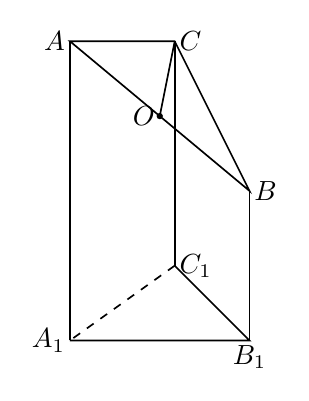
\begin{tikzpicture}[scale=0.95, semithick,
  every node/.style={inner sep=1.5pt}]

  \coordinate (A1) at (0,0);
  \coordinate (B1) at (2.4,0);
  \coordinate (C1) at (1.4,1.0);
  \coordinate (A)  at (0,4.0);
  \coordinate (B)  at (2.4,2.0);
  \coordinate (C)  at (1.4,4.0);
  \coordinate (O)  at (1.2,3.0);

  % 底面
  \draw (A1) -- (B1) -- (C1);
  \draw[dashed] (C1) -- (A1);
  % 侧棱
  \draw (A1) -- (A);
  \draw (B1) -- (B);
  \draw (C1) -- (C);
  % 截面 ABC
  \draw (A) -- (B) -- (C) -- cycle;
  % O 与 OC
  \fill (O) circle (1.2pt);
  \draw (O) -- (C);

  \node[left] at (A) {$A$};
  \node[right] at (B) {$B$};
  \node[right] at (C) {$C$};
  \node[left] at (A1) {$A_1$};
  \node[below] at (B1) {$B_1$};
  \node[right] at (C1) {$C_1$};
  \node[left] at (O) {$O$};
\end{tikzpicture}
